
\subsubsection{5.1 Main Comparison: Execution versus Pylint/Mypy (RQ1)}

Execution feedback significantly outperforms pylint/mypy feedback on both benchmarks. Figure 1 shows the pass@1 improvement delta with 95\% bootstrap confidence intervals.

\textbf{Table 1: Pass@1 by condition on HumanEval and MBPP.}

\begin{table*}[htbp]
\centering
\resizebox{\dimexpr 2\columnwidth+\columnsep\relax}{!}{%
\begin{tabular}{lllll}
\toprule
Condition & HumanEval pass@1 & $\Delta _HE$ & MBPP pass@1 & $\Delta _MBPP$ \\
\midrule
No-feedback baseline & 61.0\% & --- & 33.1\% & --- \\
Pylint/mypy repair & 56.7\% & $-4.3pp$ & 51.4\% & +18.3pp \\
Execution feedback & 65.9\% & +4.9pp & 73.3\% & +40.2pp \\
\bottomrule
\end{tabular}
}
\end{table*}

All values derived from h-m1/results/metrics.json and verified against h-e1/results/metrics.json.

The most striking result is on MBPP: a single round of execution feedback repair improves pass@1 from 33.1\% to 73.3\%, a +40.2pp absolute increase. On HumanEval, pylint/mypy repair produces a regression of 4.3pp relative to no-feedback baseline, while execution feedback improves by 4.9pp.

\textbf{Table 2: McNemar test results (execution feedback vs. pylint/mypy).}

\begin{table}[htbp]
\centering
\resizebox{\columnwidth}{!}{%
\begin{tabular}{llll}
\toprule
Benchmark & Exec-only repairs & Pylint-only repairs & McNemar p-value \\
\midrule
HumanEval & 15 & 0 & p = 0.0001 (exact) \\
MBPP & 85 & 2 & p < $10^{-18}$ (chi-square) \\
\bottomrule
\end{tabular}
}
\end{table}

McNemar contingency tables (from h-m1/results/mcnemar\_humaneval.json and mcnemar\_mbpp.json): HumanEval --- both pass: 93, exec-only pass: 15, pylint-only pass: 0, both fail: 56. MBPP --- both pass: 192, exec-only pass: 85, pylint-only pass: 2, both fail: 99.

On HumanEval, 15 problems are exclusively repaired by execution feedback; zero are exclusively repaired by pylint/mypy. On MBPP, 85 problems are exclusively repaired by execution versus 2 by pylint/mypy.

\begin{figure}[htbp]
\centering
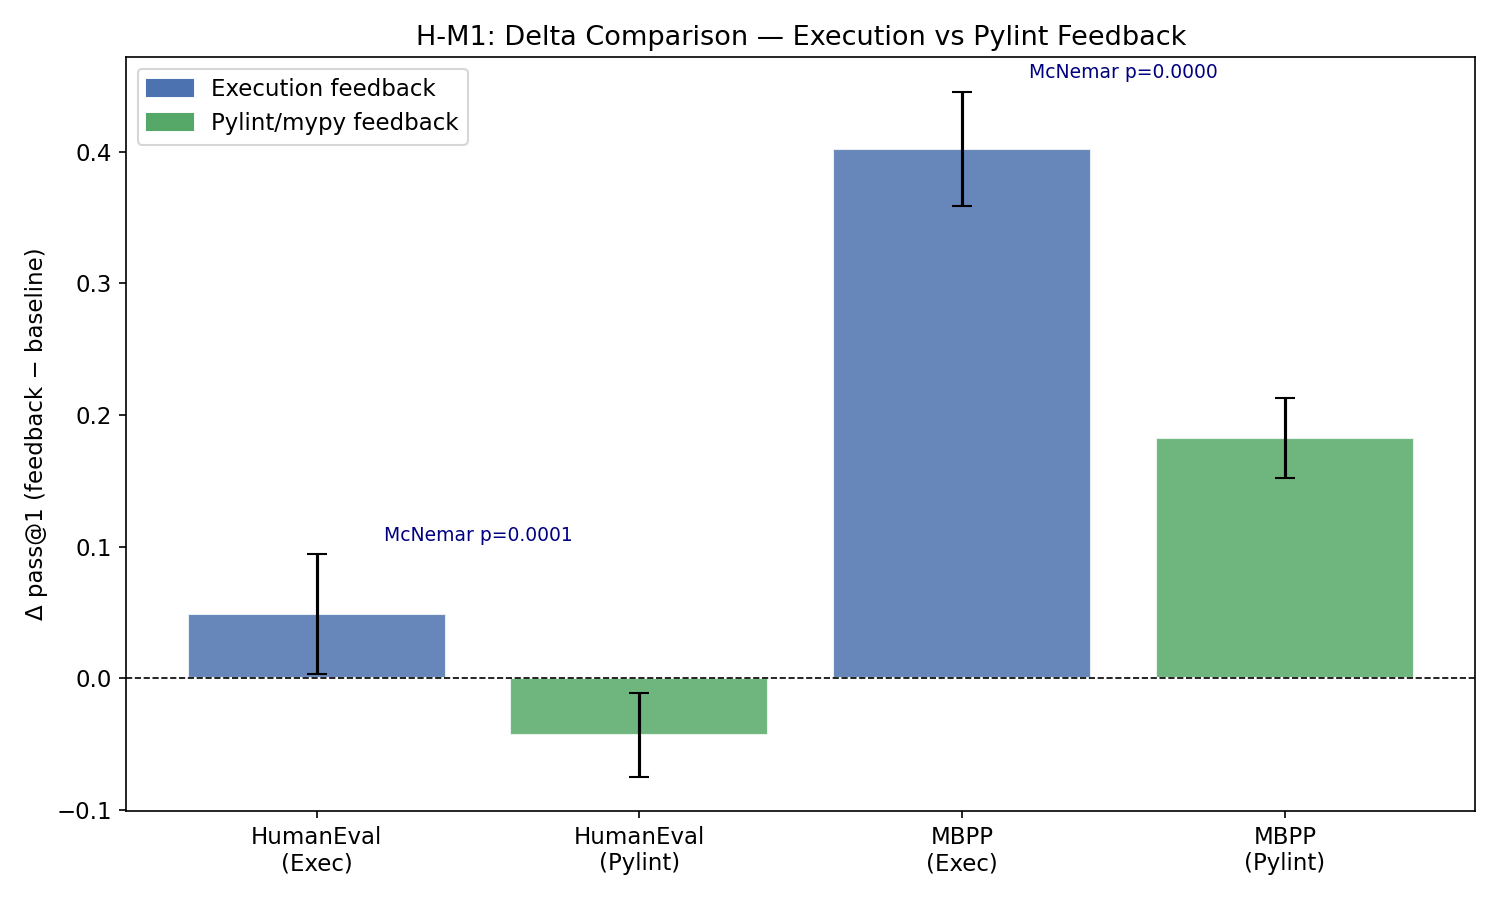
\includegraphics[width=\columnwidth]{figures/figure1_delta_comparison.png}
\caption{Figure 1: Pass@1 improvement delta with 95\% bootstrap confidence intervals and McNemar p-values}
\label{fig:figure1_delta_comparison}
\end{figure}

\textit{Figure 1: Pass@1 improvement delta ($\Delta _pass$@1 relative to no-feedback baseline) for execution feedback and pylint/mypy repair on HumanEval and MBPP, with 95\% bootstrap confidence intervals and McNemar test p-values. Execution feedback is significantly superior on both benchmarks.}

\begin{figure}[htbp]
\centering
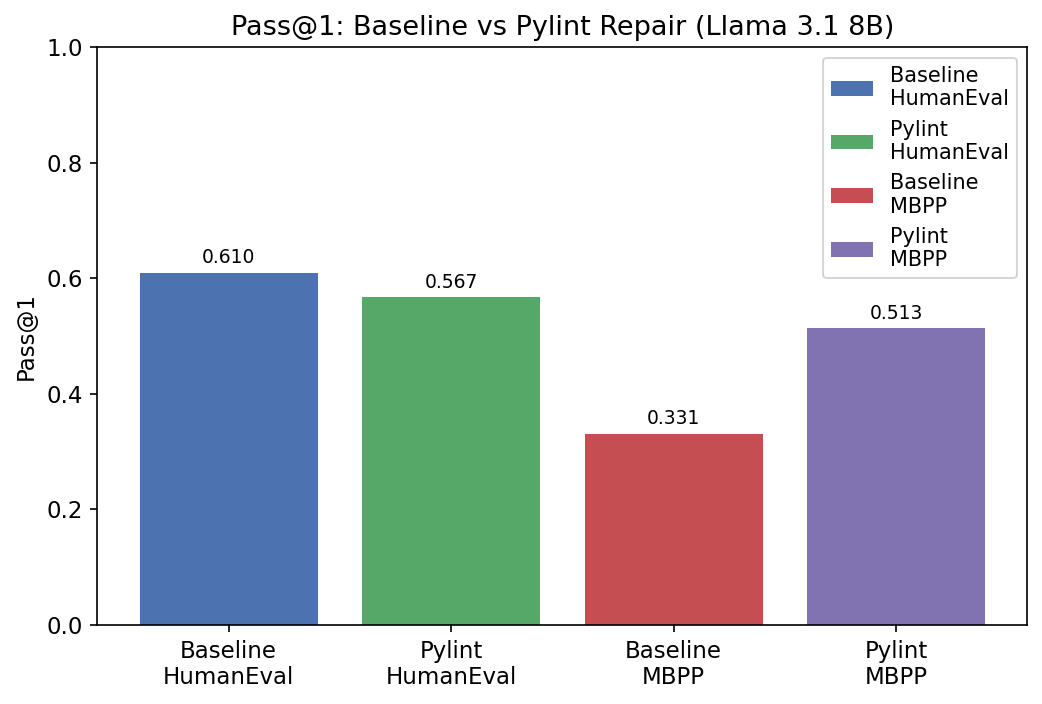
\includegraphics[width=\columnwidth]{figures/figure1_pass_at_1_comparison.png}
\caption{Figure 4: Absolute pass@1 values for all conditions}
\label{fig:figure1_pass_at_1_comparison}
\end{figure}

\textit{Figure 4: Absolute pass@1 values for baseline, pylint/mypy repair, and execution feedback conditions on HumanEval and MBPP.}

\subsubsection{5.2 Pylint/Mypy Coverage Analysis --- Mechanism (RQ2)}

\textbf{Total coverage:} Pylint/mypy flags 100\% of the 64 HumanEval baseline failures (bootstrap 95\% CI: [100\%, 100\%]).

\textbf{Table 3: Pylint flag category distribution across 64 HumanEval baseline failures (300 total flags).}

\begin{table}[htbp]
\centering
\resizebox{\columnwidth}{!}{%
\begin{tabular}{llll}
\toprule
Category & Flags & Fraction & Type \\
\midrule
C (Convention) & 283 & 94.3\% & Style (C0304, C0114) \\
R (Refactor) & 8 & 2.7\% & Structural \\
W (Warning) & 7 & 2.3\% & Functional \\
E (Error) & 1 & 0.3\% & Functional \\
I (Information) & 0 & 0.0\% & Informational \\
\bottomrule
\end{tabular}
}
\end{table}

Note: The ground truth file (065\_ground\_truth.yaml) records 1 I-category flag in the dataset; the h-m2 validation report (04\_validation.md) records 0 I-category flags in its category breakdown table. Both sources agree that I-category flags contribute 0\% of the 300 total flags reported in Table 3. The functional (E+W) coverage calculation is consistent across both sources.

\textbf{Functional coverage (E+W):} 8 of 64 HumanEval baseline failures (12.5\%) receive at least one Error or Warning category flag. The I-category flag is informational, not functional, and is excluded from functional coverage.

\textbf{Mypy coverage:} 0 of 64 HumanEval baseline failures (0\%).

The 100\% total coverage is driven by C0304 (''missing-final-newline'') and C0114 (''missing-module-docstring'') --- formatting properties of LLM code generation outputs that fire universally on any code snippet lacking a trailing newline or module docstring, regardless of whether the code is functionally correct. These flags are present on every failing solution because they are artifacts of the prompt-completion format, not indicators of functional errors.

\begin{figure}[htbp]
\centering
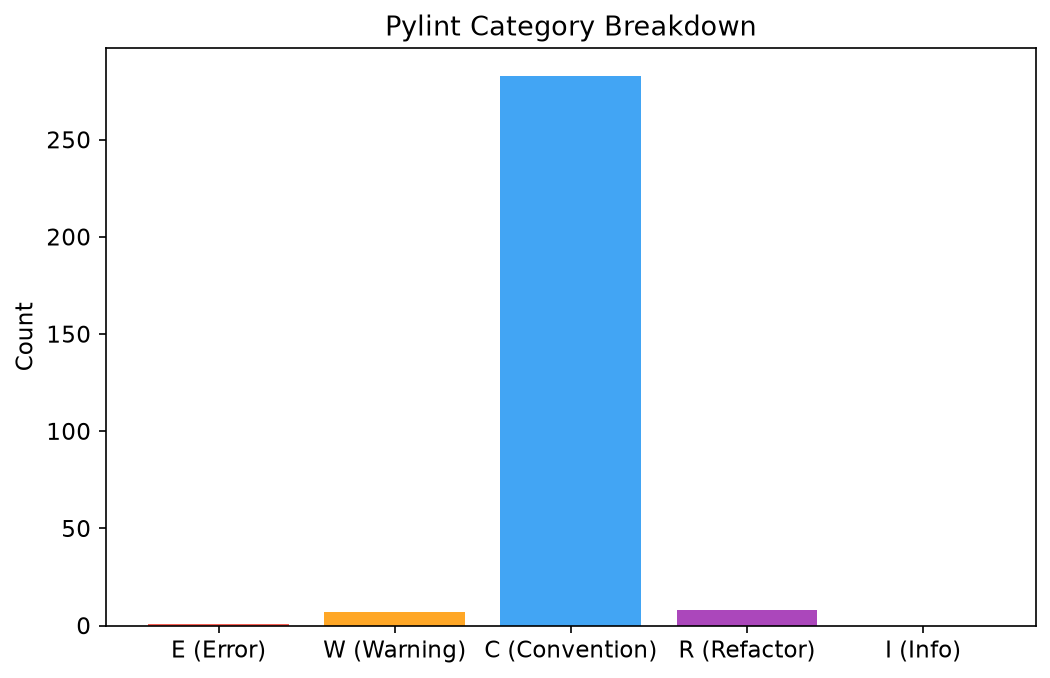
\includegraphics[width=\columnwidth]{figures/fig2_pylint_categories.png}
\caption{Figure 2: Pylint flag category distribution}
\label{fig:fig2_pylint_categories}
\end{figure}

\textit{Figure 2: Distribution of pylint flag categories across 64 HumanEval baseline failures. Convention (C) flags dominate at 94.3\%; functional Error (E) and Warning (W) categories cover only 12.5\% of failures.}

\begin{figure}[htbp]
\centering
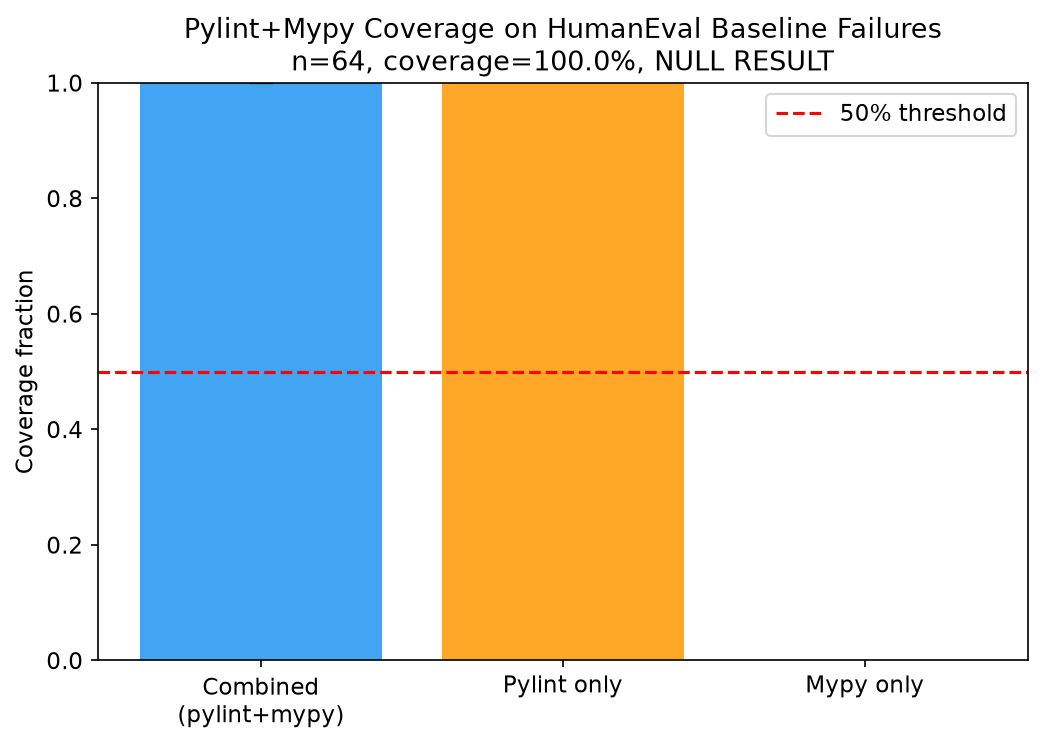
\includegraphics[width=\columnwidth]{figures/fig1_coverage_bar.png}
\caption{Figure 5: Total versus functional pylint coverage}
\label{fig:fig1_coverage_bar}
\end{figure}

\textit{Figure 5: Total pylint/mypy coverage (100\%) versus functional coverage (E+W: 12.5\%) of HumanEval baseline failures, with 95\% bootstrap confidence intervals.}

\subsubsection{5.3 Benchmark Asymmetry (RQ3)}

Pylint/mypy repair reduces HumanEval pass@1 by 4.3pp but increases MBPP pass@1 by 18.3pp. Execution feedback improves both (HumanEval: +4.9pp, MBPP: +40.2pp). The asymmetric behavior of pylint/mypy repair across the two benchmarks is consistent with task-complexity moderation: MBPP's simpler function-completion tasks may tolerate style-guided rewrites without losing logical structure, while HumanEval's algorithmic problems are sensitive to structural changes triggered by style feedback.

\subsubsection{5.4 Per-Round Trajectory and Budget Saturation}

At B=1000 output tokens, the token budget is effectively exhausted after the initial generation plus one repair round for most problems. Per-round pass@1 trajectory data from h-m1 (execution condition) shows incremental improvements of 0.097 (HumanEval) and 0.601 (MBPP) in round 1; rounds 2 and 3 contribute zero incremental improvement. Results therefore characterize single-round repair performance at B=1000.

Note: The initial pass@1 recorded in round 0 of the execution feedback condition (0.622 on HumanEval) differs slightly from the no-feedback baseline (0.610). This difference arises from minor prompt-context differences between the repair loop run (which instruments all problems, including those that pass) and the standalone single-pass baseline run; it does not represent a methodological inconsistency. The no-feedback baseline (61.0\%) is reported from the standalone single-pass condition without any repair loop instrumentation.

\begin{figure}[htbp]
\centering
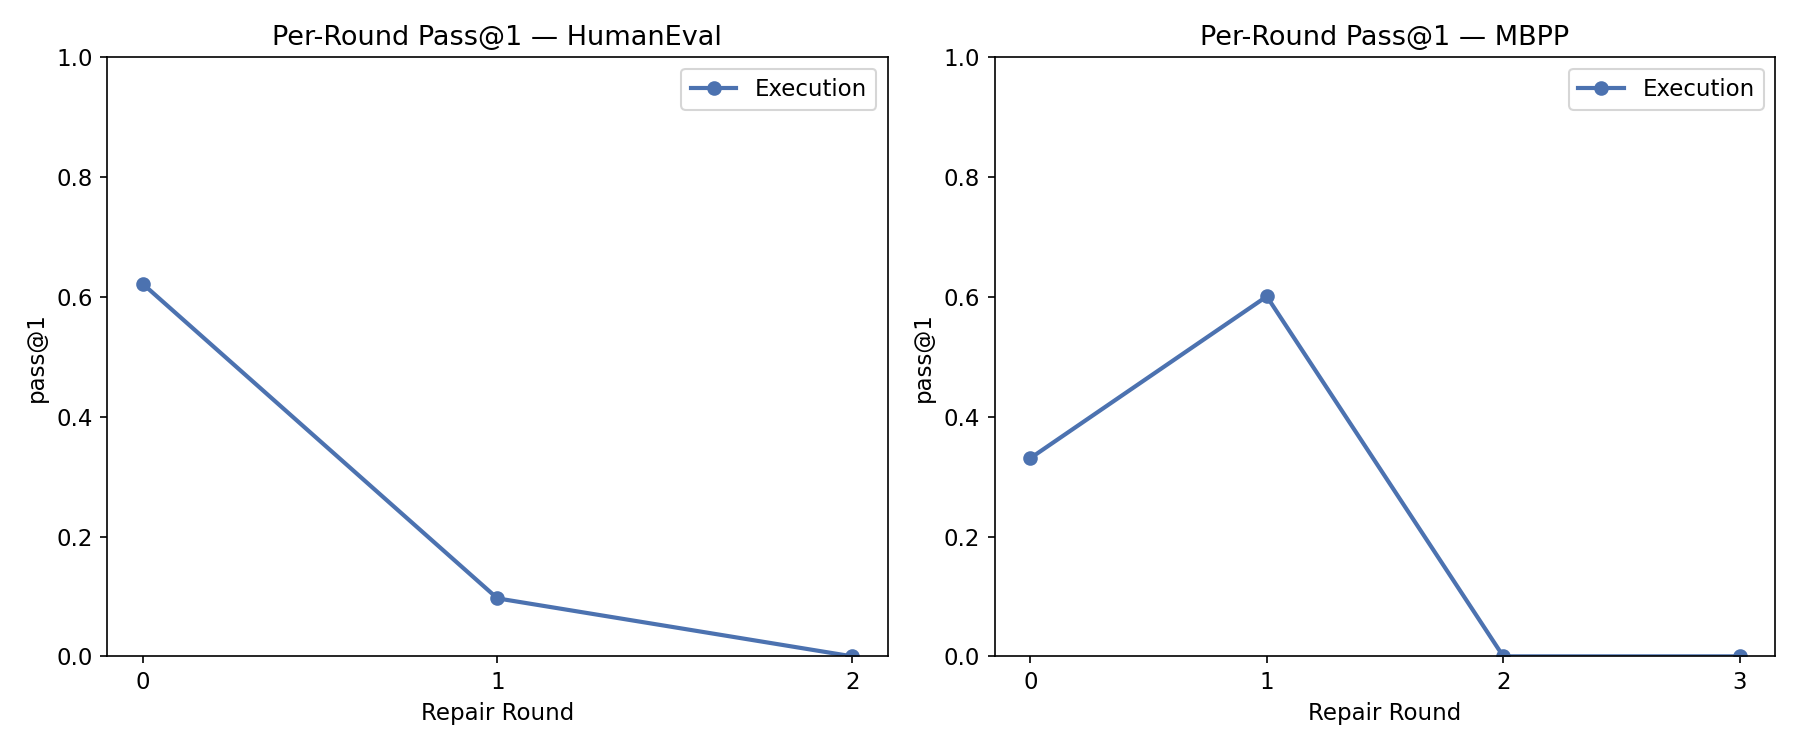
\includegraphics[width=\columnwidth]{figures/figure2_per_round_trajectory.png}
\caption{Figure 3: Per-round pass@1 trajectory}
\label{fig:figure2_per_round_trajectory}
\end{figure}

\textit{Figure 3: Per-round pass@1 trajectory for execution feedback on HumanEval and MBPP. Most improvement occurs in round 1; rounds 2 and 3 contribute near-zero incremental improvement at B=1000.}

